\documentclass[a4paper]{article}

\usepackage{graphicx}
\usepackage{amsmath,amssymb}
\usepackage{minted}
\usepackage{multirow}
\usepackage{float}
\usepackage{todonotes}
\usepackage{forest}
\usepackage{xstring}
\usepackage{xcolor}
\usepackage[most]{tcolorbox}
\usepackage{xparse}
\usepackage{natbib}

\usetikzlibrary{graphs,graphdrawing}
\usegdlibrary{layered}

% for external graphviz
\input{/home/donkarlo/Dropbox/repo/nd_ai_project/src/nd_ai/knoweldge_representation/language/formal/computer/programming/tex/latex/code_clips/external_graphviz.tex}

% for tags
\input{/home/donkarlo/Dropbox/repo/nd_ai_project/src/nd_ai/knoweldge_representation/language/formal/computer/programming/tex/latex/parts/control_sequence/kind/semtag/semtag.tex}

% for links
\input{/home/donkarlo/Dropbox/repo/nd_ai_project/src/nd_ai/knoweldge_representation/language/formal/computer/programming/tex/latex/code_clips/seehere.tex}

\title{3D City Meshes and Photorealistic 3D Tiles}
\date{}
\author{Mohammad Rahmani}

\begin{document}
    \maketitle
    
    
    \section{3D City Meshes and Photorealistic 3D Tiles}
        Three-dimensional city meshes represent buildings, terrain, and sometimes vegetation as textured geometry that can be inspected from arbitrary viewpoints.
        They can support roof-height estimation, slope analysis, orientation measurement, visibility checks, and separation of adjacent roof planes.
        Photorealistic tiles are particularly useful when roof shape must be interpreted together with surrounding structures and elevation context.
        Their limitations include mesh artefacts, stretched textures, variable level of detail, large data volumes, and licensing or access restrictions for some providers.
        Relevant platforms include Cesium ion \seeherefooter{https://ion.cesium.com/} and the City of Vienna geodata services \seeherefooter{https://www.wien.gv.at/stadtentwicklung/stadtvermessung/geodaten/}.
        
        \begin{figure}[H]
            \centering
            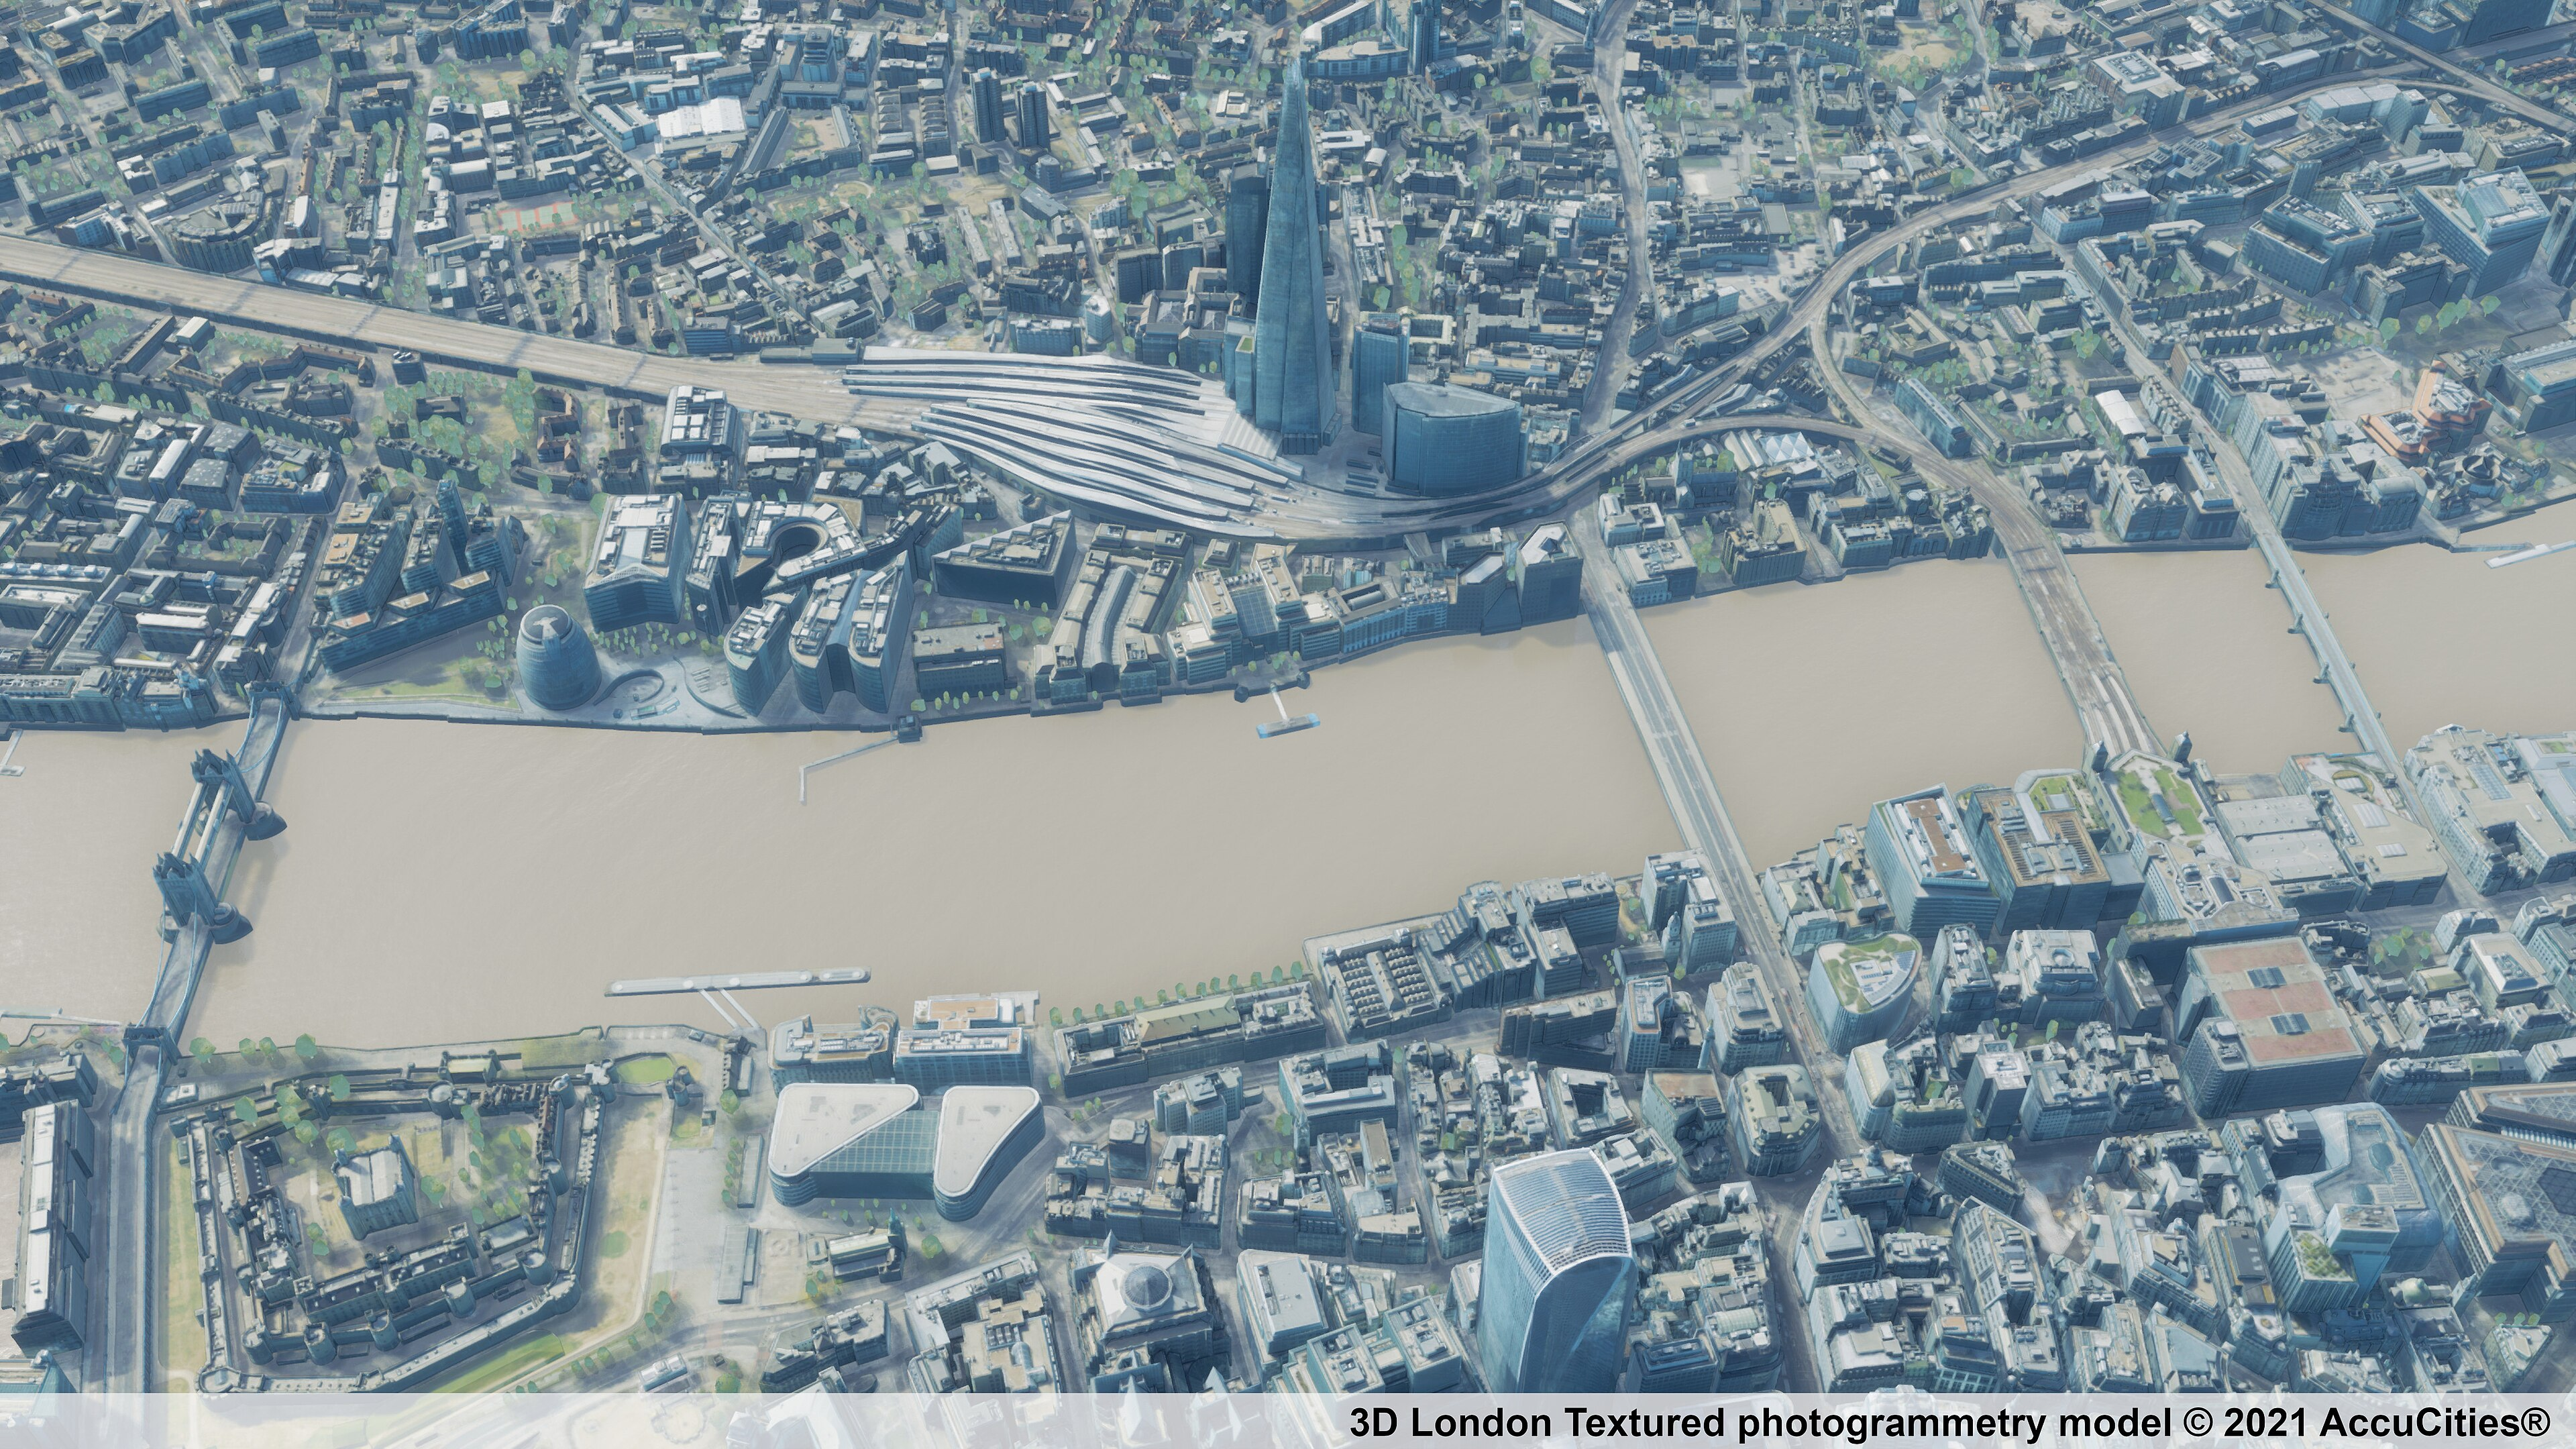
\includegraphics[width=0.9\textwidth]{images/city_3d_meshes_and_tiles_example.jpg}
            \caption{Example of a textured photogrammetric 3D city model.}
        \end{figure}
        \noindent\small Image source and licence information: \seeherefooter{https://commons.wikimedia.org/w/index.php?oldid=1035491763}.\normalsize
        
%        \bibliographystyle{plainnat}
%        \bibliography{/home/donkarlo/Dropbox/repo/nd_shared_research/bibliography/bibliography.bib}
\end{document}
